%% 
%% Latex template to System Architecture Document
%% Author: Dario A. Palminio
%% LaTeX version 2.0
%% OS: Ubuntu
%% Editor: LaTeXila 2.4.0
%% 

\documentclass[a4paper,11pt]{book}
\usepackage[T1]{fontenc}
\usepackage[utf8]{inputenc}
\usepackage{lmodern}
\usepackage{graphicx}

\graphicspath{ {images/} }

\title{System Architecture}
\author{Dario A. Palminio}

\begin{document}

\maketitle

Documentation control

%% Document Version Control (Table)
\begin{table}[h]
\begin{tabular}{lllll}
\cline{1-4}
\multicolumn{1}{|l|}{Date}       & \multicolumn{1}{l|}{Author}         & \multicolumn{1}{l|}{Version} & \multicolumn{1}{l|}{Detail}   &  \\ \cline{1-4}
\multicolumn{1}{|l|}{05/12/2014} & \multicolumn{1}{l|}{Dario Palminio} & \multicolumn{1}{l|}{1.0}     & \multicolumn{1}{l|}{Creation} &  \\ \cline{1-4}
                                 &                                     &                              &                               &  \\
                                 &                                     &                              &                               & 
\end{tabular}
\end{table}
%% 

\tableofcontents

\chapter{Introduction}

The following software has as purpose to solve a single problem. It has been done as a practical example.
This project is just a example of a simple project made in Eclipse IDE. 
The problem to resolve is following:
Build a program that performs the following operations: 
1-That receives as input a list of numbers and returns a list of prime numbers. 
2- That receives as input a file name (with word list) and returns a list of palindromes (palíndromos). 
3- Make unit tests.

\section{Purpose of the document}
This document shows the general architecture as example.

\section{Audience}
Anyone interested.

\chapter{Architecture}
% text

\section{Scope and Context}

Example.

\section{High-level Architecture}
% text

\begin{figure}[h] % Diagram
  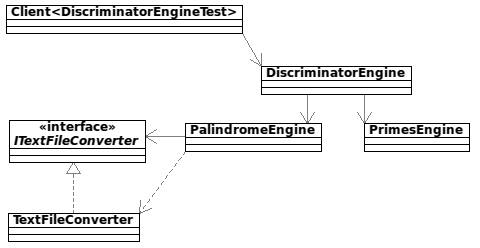
\includegraphics{general_class_diagram}
  \caption{Context Diagram}
  \centering
  \label{fig:context} %\ref{fig:context}
\end{figure}

\end{document}
